\documentclass[a4paper,12pt]{article}
\usepackage[utf8]{inputenc}
\usepackage[spanish]{babel}
\usepackage{color}
\usepackage{parskip}
\usepackage{graphicx}
\usepackage{multirow}
\usepackage{listings}
\usepackage{vmargin}
\usepackage{datetime}
\newdate{date}{14}{09}{2017}
\graphicspath{ {imagenes/} }
\definecolor{mygreen}{rgb}{0,0.6,0}
\definecolor{lbcolor}{rgb}{0.9,0.9,0.9}
\usepackage{epstopdf}
\usepackage{float}


\setpapersize{A4}
\setmargins{2.5cm}       % margen izquierdo
{1.5cm}                        % margen superior
{16.5cm}                      % anchura del texto
{23.42cm}                    % altura del texto
{10pt}                           % altura de los encabezados
{1cm}                           % espacio entre el texto y los encabezados
{0pt}                             % altura del pie de página
{2cm}     

\lstset{
backgroundcolor=\color{lbcolor},
    tabsize=4,    
%   rulecolor=,
    language=[GNU]C++,
        basicstyle=\tiny,
        aboveskip={1.5\baselineskip},
        columns=fixed,
        showstringspaces=false,
        extendedchars=false,
        breaklines=true,
        prebreak = \raisebox{0ex}[0ex][0ex]{\ensuremath{\hookleftarrow}},
        frame=single,
        showtabs=false,
        showspaces=false,
        showstringspaces=false,
        identifierstyle=\ttfamily,
        keywordstyle=\color[rgb]{0,0,1},
        commentstyle=\color[rgb]{0.026,0.112,0.095},
        stringstyle=\color{red},
        numberstyle=\color[rgb]{0.205, 0.142, 0.73},
%        \lstdefinestyle{C++}{language=C++,style=numbers}’.
}


\begin{document}
\title{Final de la Práctica 2}
\author{
Christofer Fabián Chávez Carazas \\
\small{Universidad Nacional de San Agustín de Arequipa} \\
\small{Escuela Profesional de Ciencia de la Computación} \\
\small{Computación Centrada en Redes}
}
\date{\displaydate{date}}

\maketitle

\begin{large}
 \textbf{Actividades}
\end{large}

 
 \begin{figure}[H]
  \centering
  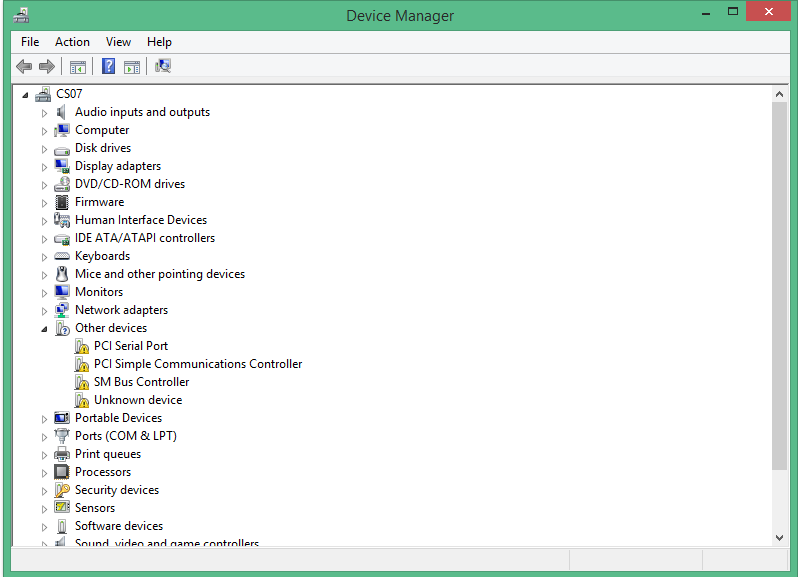
\includegraphics[scale = 0.5]{1.png}
  \caption{Administrador de Dispositivos}
 \end{figure}
 
 \begin{figure}[H]
  \centering
  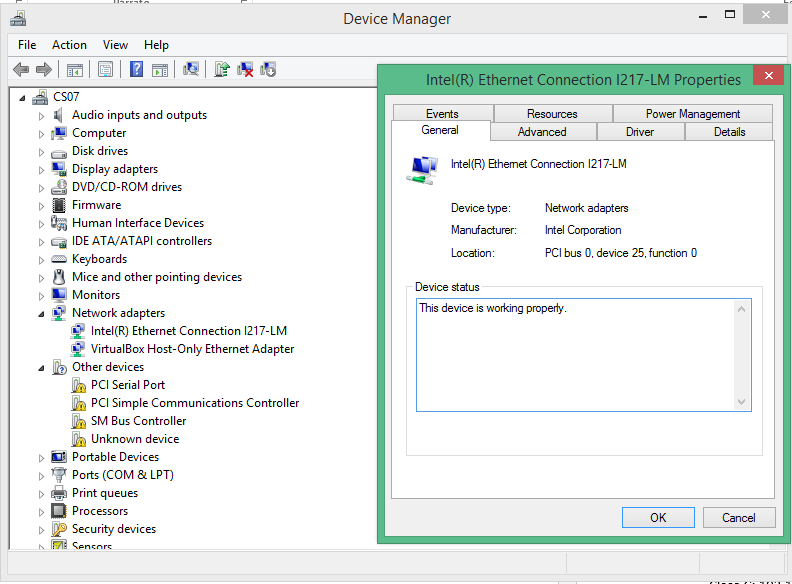
\includegraphics[scale = 0.5]{2.png}
  \caption{Propiedades del dispositivo de Ethernet}
 \end{figure}
 
 \begin{figure}[H]
  \centering
  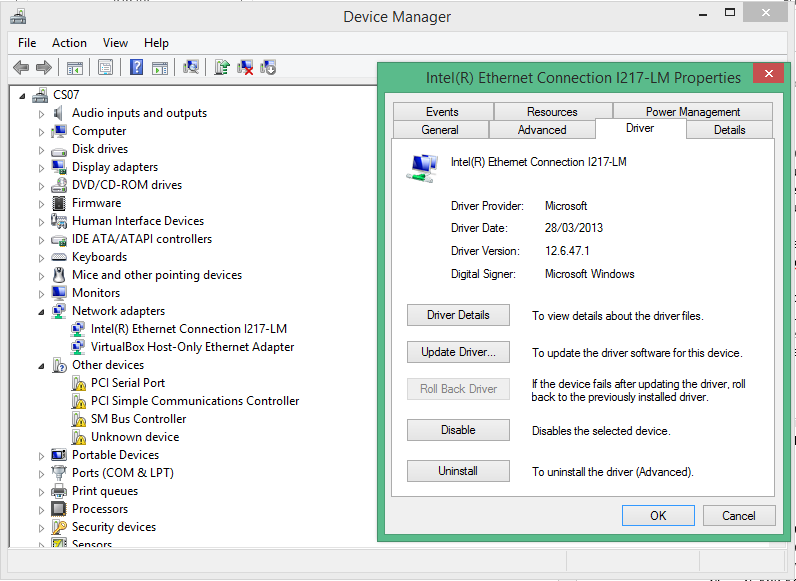
\includegraphics[scale = 0.5]{3.png}
  \caption{Driver del dispositivo de Ethernet}
 \end{figure}

 \begin{figure}[H]
  \centering
  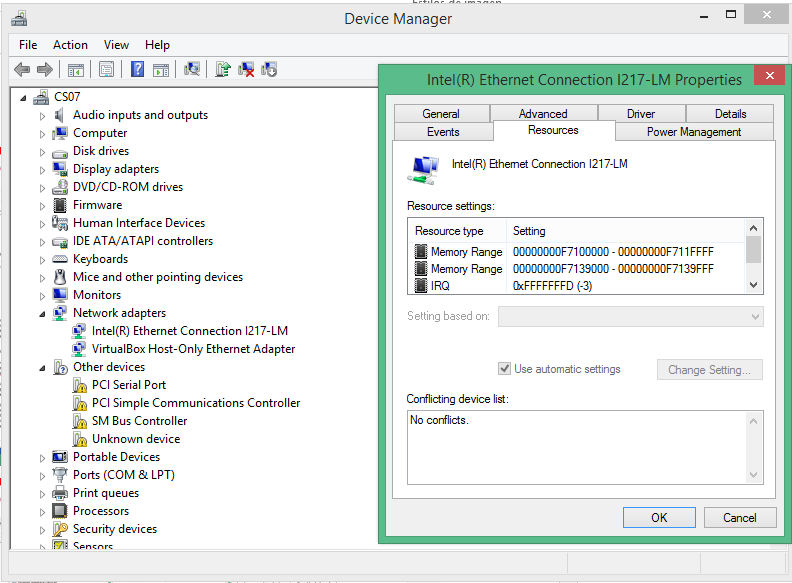
\includegraphics[scale = 0.5]{4.png}
  \caption{Recursos del dispositivo de Ethernet}
 \end{figure}
 
 \begin{figure}[H]
  \centering
  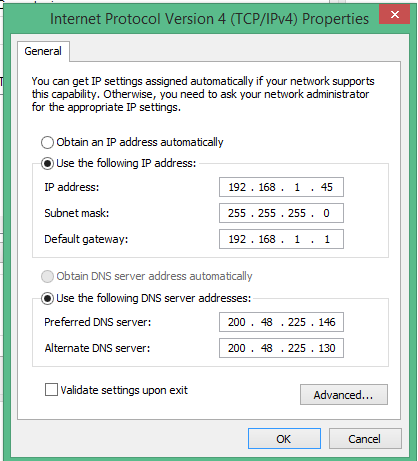
\includegraphics[scale = 0.5]{5.png}
  \caption{IP original de la máquina}
 \end{figure}
 
 \begin{figure}[H]
  \centering
  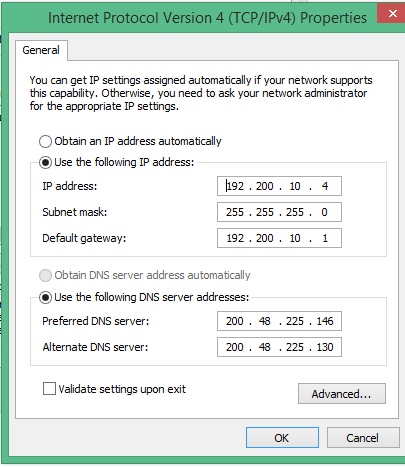
\includegraphics[scale = 0.5]{6.png}
  \caption{IP de tipo C}
 \end{figure}
 
 \begin{figure}[H]
  \centering
  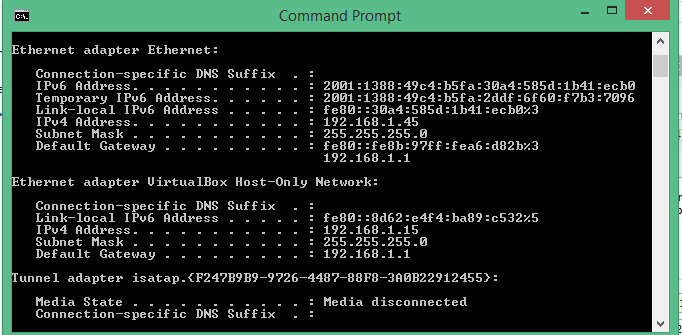
\includegraphics[scale = 0.5]{7.png}
  \caption{Comando ipconfig con la ip de la máquina original}
 \end{figure}
 
 \begin{figure}[H]
  \centering
  
\includegraphics[scale = 0.5]{8.png}
  \caption{Comando ipconfig con la ip de tipo C}
 \end{figure}
 
 \begin{figure}[H]
  \centering
  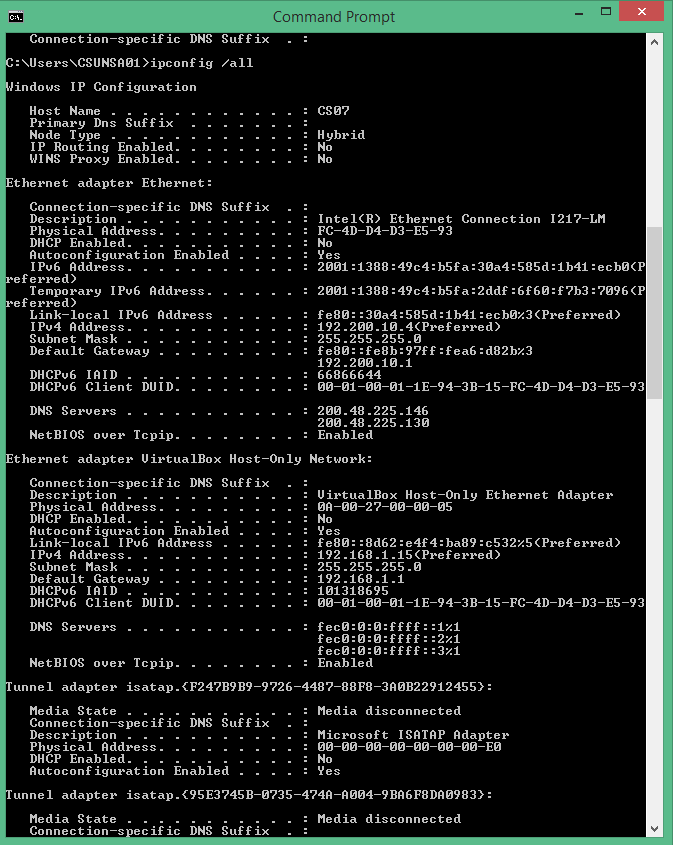
\includegraphics[scale = 0.5]{9.png}
  \caption{Comando ipconfig /all}
 \end{figure}
 
 \begin{figure}[H]
  \centering
  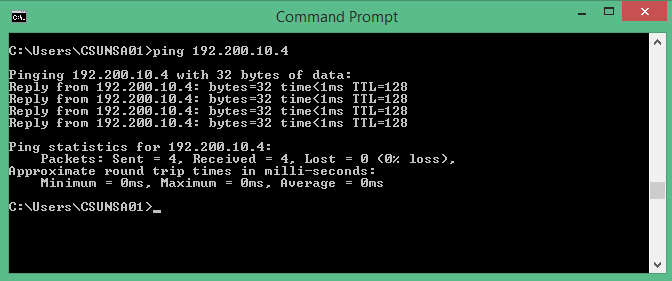
\includegraphics[scale = 0.5]{10.png}
  \caption{Ping a la IP 192.200.10.4 (mi misma IP)}
 \end{figure}
 
 \begin{figure}[H]
  \centering
  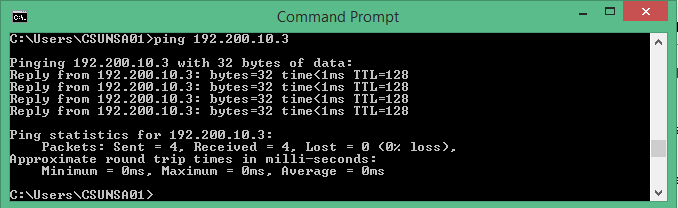
\includegraphics[scale = 0.5]{11.png}
  \caption{Ping a otra PC}
 \end{figure}
 
 \begin{figure}[H]
  \centering
  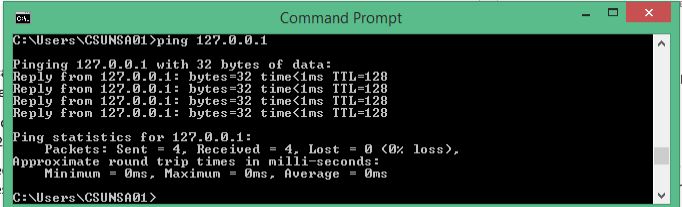
\includegraphics[scale = 0.5]{12.png}
  \caption{Pina a la IP localhost}
 \end{figure}
 
 \begin{figure}[H]
  \centering
  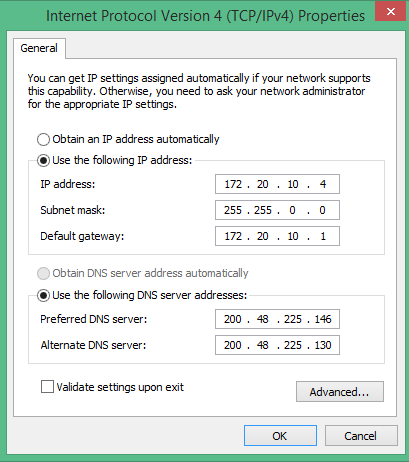
\includegraphics[scale = 0.5]{13.png}
  \caption{IP de tipo B}
 \end{figure}
 
 \begin{figure}[H]
  \centering
  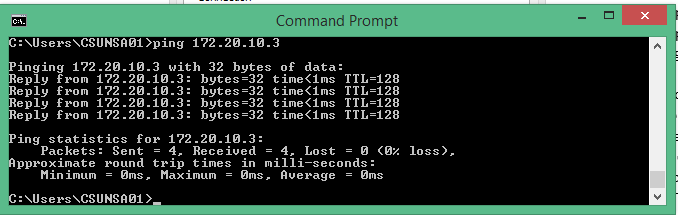
\includegraphics[scale = 0.5]{14.png}
  \caption{Ping a otra PC}
 \end{figure}
 
 \begin{figure}[H]
  \centering
  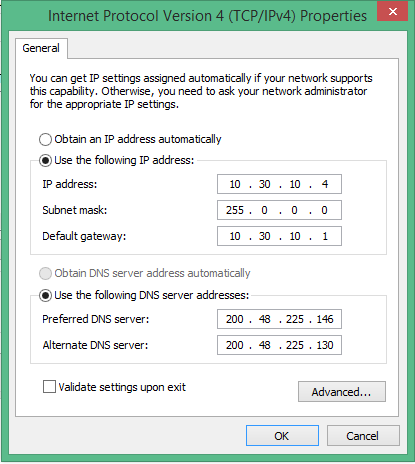
\includegraphics[scale = 0.5]{15.png}
  \caption{IP de tipo A}
 \end{figure}
 
 \begin{figure}[H]
  \centering
  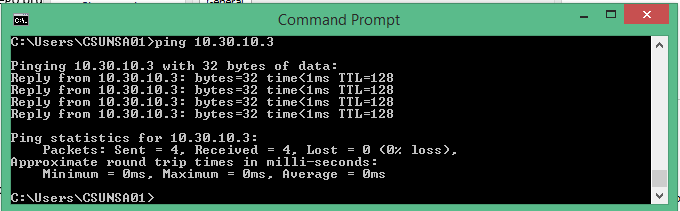
\includegraphics[scale = 0.5]{16.png}
  \caption{Ping a otra PC}
 \end{figure}
 
 \begin{figure}[H]
  \centering
  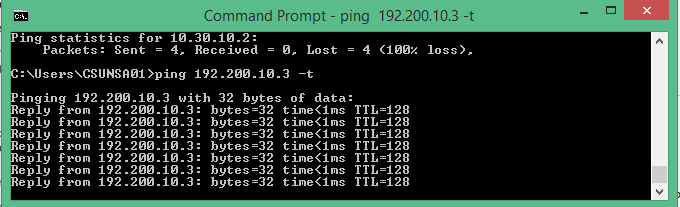
\includegraphics[scale = 0.5]{17.png}
  \caption{Ping a otra PC de forma constante}
 \end{figure}
 
 \begin{figure}[H]
  \centering
  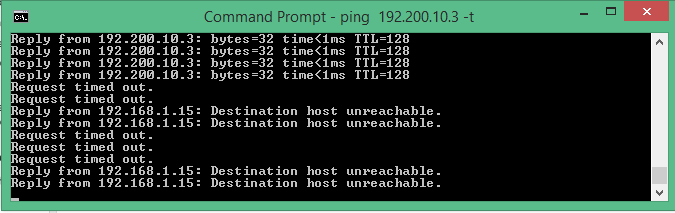
\includegraphics[scale = 0.5]{18.png}
  \caption{Ping constante sin una conexión}
 \end{figure}
 
 \begin{figure}[H]
  \centering
  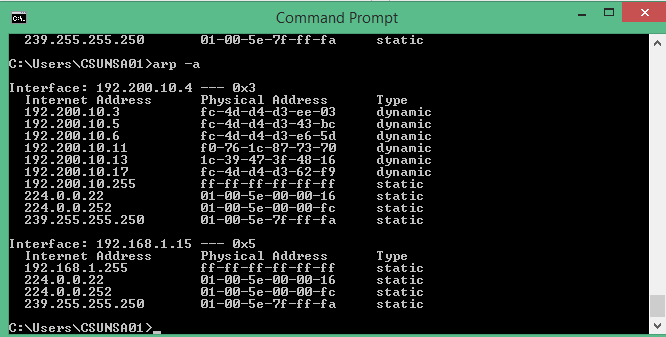
\includegraphics[scale = 0.5]{19.png}
  \caption{Lista ARP}
 \end{figure}
 
 \begin{figure}[H]
  \centering
  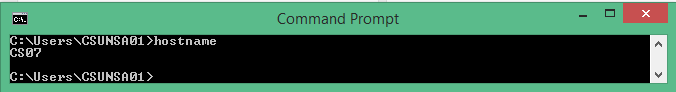
\includegraphics[scale = 0.5]{20.png}
  \caption{Comando hostname}
 \end{figure}
 
 \begin{figure}[H]
  \centering
  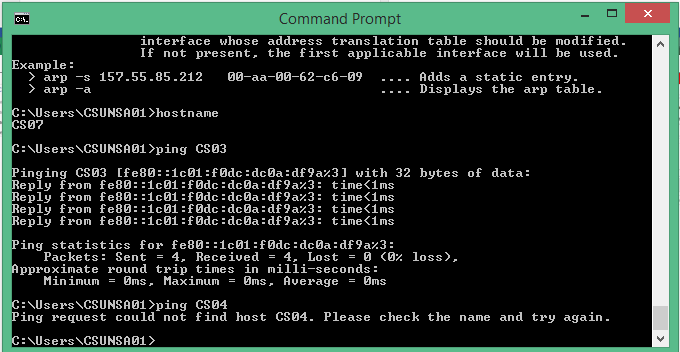
\includegraphics[scale = 0.5]{21.png}
  \caption{Ping a otra PC con el hostname}
 \end{figure}
 
\begin{large}
 \textbf{Cuestionarios}
\end{large}

\begin{enumerate}
 \item \textbf{Mostrar el proceso para compartir una carpeta en Windows}
 
 Antes de nada, se debe tener configurada una red para poder compartir cualquier carpeta.
 \begin{itemize}
  \item Hacer click derecho en la carpeta que se quiera compartir y seleccionar \textit{Propiedades}.
  \item Entrar en la pestaña \textit{Compartir} y hacer click en el botón del mismo nombre.
  \item En la pantalla siguiente se debe elegir a que usuarios se va a compartir la carpeta, elegir todos.
  \item En esa misma pantalla se debe definir los permisos de los usuarios a los que se les va a compartir la carpeta. Se 
  puede elegir permisos de Lectura y permisos de Lectura y Escritura.
  \item Hacer click en Aceptar.
 \end{itemize}

 \item \textbf{Mostrar el proceso para compartir una impresora en Windows}
 
 \begin{itemize}
  \item Ir a Dispositivos e Impresoras.
  \item Hacer click derecho en la impresora que se quiera compartir y elegir Propiedades de Impresora.
  \item Entrar en la pestaña \textit{Compartir}.
  \item Hacer click en \textit{Compartir esta impresora}, luego en aplicar y aceptar.
 \end{itemize}
 
 \item \textbf{Explique los tipos de redes según el protocolo IP.
 Qué clase de dirección IP utilizó al inicio. Qué mensaje se obtiene a una dirección IP que no existe.}

 Existen cinco clases de redes, A, B, C, D y E, de las cuales solo las tres primeras se utilizan.
 \begin{itemize}
  \item En una red de clase A, se asigna el primer octeto para identificar la red, reservando los tres últimos octetos (24 bits) para que sean asignados a los hosts, de modo que la cantidad máxima de hosts es 224 - 2 (excluye la dirección reservada para broadcast (últimos octetos en 255) y de red (últimos octetos en 0)), es decir, 16 777 214 hosts.
  \item En una red de clase B, se asignan los dos primeros octetos para identificar la red, reservando los dos octetos finales (16 bits) para que sean asignados a los hosts, de modo que la cantidad máxima de hosts por cada red es $2^{16}$ - 2, o 65 534 hosts.
  \item En una red de clase C, se asignan los tres primeros octetos para identificar la red, reservando el octeto final (8 bits) para que sea asignado a los hosts, de modo que la cantidad máxima de hosts por cada red es 28 - 2, o 254 hosts.
 \end{itemize}

 \item \textbf{¿Qué es la dirección MAC y cómo se obtiene?}
 
 La dirección MAC(\textit{Media Acces Control}) es un identificador de 48 bits que corresponde de forma única a una tarjeta o 
 dispositivo de red. Las direcciones MAC son únicas a nivel mundial, puesto que son escritas directamente, en forma binaria,
 en el hardware en su momento de fabricación. Debido a esto, las direcciones MAC son a veces llamadas \textit{burned-in addresses}, en inglés.
 La dirección MAC se puede obtener con el comando ipconfig /all.
 
 \item \textbf{¿Pueden existir dos hosts con la misma dirección IP? ¿Por qué?
 ¿Un host puede tener más de una dirección IP?, si fuese así muestre el procedimiento}
 
 No puede haber dos host con la misma IP porque sino, al intentar enviar cosas habría colisión de datos y al intentar recibir datos
 no se sabría para que host es el mensaje. Al mismo tiempo un host no puede tener más de una dirección IP. Pero si esta cambia dinámicamente
 después de un periodo de tiempo.
 
 \item \textbf{Suponiendo que se esté usando un servidor DHCP, ¿cómo se libera y obtiene una nueva dirección IP?}
 
 El cliente y el servidor se comunican mediante varios paquetes DHCP, estos pueden ser los siguientes:
 \begin{itemize}
  \item \textbf{DHCPDISCOVER:} para ubicar servidores DHCP disponibles.
  \item \textbf{DHCPOFFER:} respuesta del servidor a un paquete DHCPDISCOVER, que contiene los parámetros iniciales.
  \item \textbf{DHCPREQUEST:} solicitudes varias del cliente, por ejemplo, para extender su concesión.
  \item \textbf{DHCPACK:} respuesta del servidor que contiene los parámetros y la dirección IP del cliente.
  \item \textbf{DHCPNAK:} respuesta del servidor para indicarle al cliente que su concesión ha vencido o si el cliente anuncia una configuración de red errónea.
  \item \textbf{DHCPDECLINE:} el cliente le anuncia al servidor que la dirección ya está en uso.
  \item \textbf{DHCPRELEASE:} el cliente libera su dirección IP.
  \item \textbf{DHCPINFORM:} el cliente solicita parámetros locales, ya tiene su dirección IP.
 \end{itemize}

 El primer paquete emitido por el cliente es un paquete del tipo DHCPDISCOVER. El servidor responde con un paquete DHCPOFFER,
 fundamentalmente para enviarle una dirección IP al cliente. El cliente establece su configuración y luego realiza un
 DHCPREQUEST para validar su dirección IP (una solicitud de transmisión ya que DHCPOFFER no contiene la dirección IP)
 El servidor simplemente responde con un DHCPACK con la dirección IP para confirmar la asignación. Normalmente,
 esto es suficiente para que el cliente obtenga una configuración de red efectiva, pero puede tardar más o menos en función
 de que el cliente acepte o no la dirección IP. 
 
 \item \textbf{¿Qué se entiende como Dirección de Red y cómo se obtiene?}
 
 La dirección de red es la utilizada para referirse a una red. Esta se obtiene haciendo una operación AND entre una dirección IP
 y la máscara de red.
 
 \item \textbf{¿Qué significa el parámetro TTL del comando ping y qué función tiene?}
 
 TTL (tiempo de vida) especifica el tiempo de vida de los paquetes enviados. Es usado para indicar por cuántos nodos
 puede pasar un paquete antes de ser descartado por la red o devuelto a su origen.
 
 \item \textbf{¿Qué significa la dirección IP 127.0.0.1 y cómo se le denomina?. Detalle si existen otras direcciones IP reservadas}
 
 La dirección 127.0.0.1 o llamada también localhost, es usada para referirse al mismo host. Si se envía un paquete a esta dirección, este nunca
 sale de la computadora, sino va directo a la tarjeta de red. Otras IPs reservadas son la dirección de red y la dirección de broadcast.
 
 \item \textbf{¿Cuál es la diferencia entre un eco a 127.0.0.1 y el eco a su propia dirección?}
 
 En que el eco a 127.0.0.1, el paquete nunca llega a salir del host, de frente va a la tarjeta de red, y el eco a su propia
 dirección IP, el paquete si sale del host, pasea por la red, y regresa nuevamente al host.
 
 \item \textbf{Presente un breve resumen de al menos dos comandos TCP/IP}
 
 \textbf{IpConfig}
 
 Este comando muestra la dirección IP activa, la mascara de red así coma la puerta de enlace predeterminada a nivel de las interfaces
 de red conocidas en el equipo local.
 \begin{itemize}
  \item \textbf{/all:} Muestra toda la configuración de la red, incluyendo los servidores DNS, WINS, bail DHCP, etc ...
  \item \textbf{/renew [tarjeta]:} Renueva la configuración DHCP de todas las tarjetas o de una tarjeta específica si utiliza el parámetro tarjeta.
  \item \textbf{/release [tarjeta]:} Envía un mensaje DHCPRELEASE al servidor DHCP para liberar la configuración DHCP actual y anular la configuración IP de todas las tarjetas.
 \end{itemize}
 
 \textbf{Arp}
 
 ARP: Resolución de direcciones IP en direcciones MAC. Muestra y modifica las tablas de traducción de direcciones IP a direcciones Físicas utilizadas por el protocolo de resolución de dirección (ARP). 
 
 \begin{itemize}
  \item \textbf{-a} Muestra las entradas ARP activas interrogando al protocolo de datos activos.
  \item \textbf{-d} Borra al host especificado por adr\_inet.
  \item \textbf{-s} Agrega al host y relaciona la dirección Internet adr\_inet a la Física adr\_eth.
 \end{itemize}
 
 \item \textbf{Describa claramente la diferencia entre IPv4 e IPv6}
 
 La única gran diferencia es que la IPv6 extiende la IPv4 ya que esta se quedó corta. La IPv6 asigna 128 bits a cada IP
 en vez de sólo 32 como la IPv4.
 
 \item \textbf{Describa la forma de obtener la dirección MAC de otros dos tipos de dispositivos (ejemplo teléfono celular, televisor, modem, etc)}
 
 Al ser la dirección MAC única en todos los dispositivos y nunca cambia, se puede obtener fácilmente de otros dispositivos
 viendo su configuración de red en sus opciones, o en otros dispositivos, viendo la configuración del fabricante.
 


 
 
 
\end{enumerate}

\end{document}

